\documentclass[border=3pt]{standalone}
% Preâmbulo compartilhado pelos diagramas TikZ da aula 13 (SLAM com EKF)
\usepackage[T1]{fontenc}
\usepackage[utf8]{inputenc}
\usepackage{lmodern}
\usepackage{amsmath}
\usepackage{xcolor}
\usepackage{tikz}
\usetikzlibrary{arrows.meta,angles,quotes,decorations.pathmorphing,decorations.pathreplacing,calc,
                positioning,shapes.geometric,shapes.misc,backgrounds,fit,
                math}

% Paleta (mesma dos SVGs originais)
\definecolor{dblue}{HTML}{2A5B8C}
\definecolor{dorange}{HTML}{B3541E}
\definecolor{dgreen}{HTML}{4A7C59}
\definecolor{dred}{HTML}{9C4B4B}
\definecolor{dcream}{HTML}{F4F1EA}
\definecolor{dshade}{HTML}{DDD7C9}

% Função gaussiana (não normalizada por padrão de escala visual)
\pgfmathdeclarefunction{gauss}{3}{%
  \pgfmathparse{1/(#3*sqrt(2*pi))*exp(-((#1-#2)^2)/(2*#3^2))}%
}

% Estilos comuns (prefixo d... para não colidir com chaves internas do pgf)
\tikzset{
  >={Stealth[length=2mm]},
  dguide/.style={gray!55, dashed, line width=0.4pt},
  daxis/.style={gray!60, line width=0.7pt, ->},
  dbody/.style={fill=black!3, draw=black!80, line width=1pt},
  dacc/.style={draw=dblue, line width=1pt},
  dlbl/.style={black!55, font=\small},
  dsub/.style={black!45, font=\footnotesize},
  dstate/.style={circle, draw=black!80, fill=dcream, line width=1pt,
                 minimum size=17mm, font=\large, inner sep=1pt},
  dobs/.style={circle, draw=black!80, fill=dshade, line width=1pt,
               minimum size=14mm, font=\large, inner sep=1pt},
  dbox/.style={rounded corners=2pt, draw=black!80, fill=dcream, line width=1pt,
               align=center, inner sep=6pt},
  dop/.style={circle, draw=black!80, fill=white, line width=1pt,
              minimum size=6mm, inner sep=0pt, font=\small},
  dtrans/.style={->, dblue, line width=1pt},
  dmeas/.style={->, dorange, line width=1pt},
  dcurve/.style={line width=1pt, dblue},
  dcurveb/.style={line width=1.4pt, dorange},
}

\begin{document}
\hyphenpenalty=10000 \exhyphenpenalty=10000 \tolerance=9999 \emergencystretch=3em
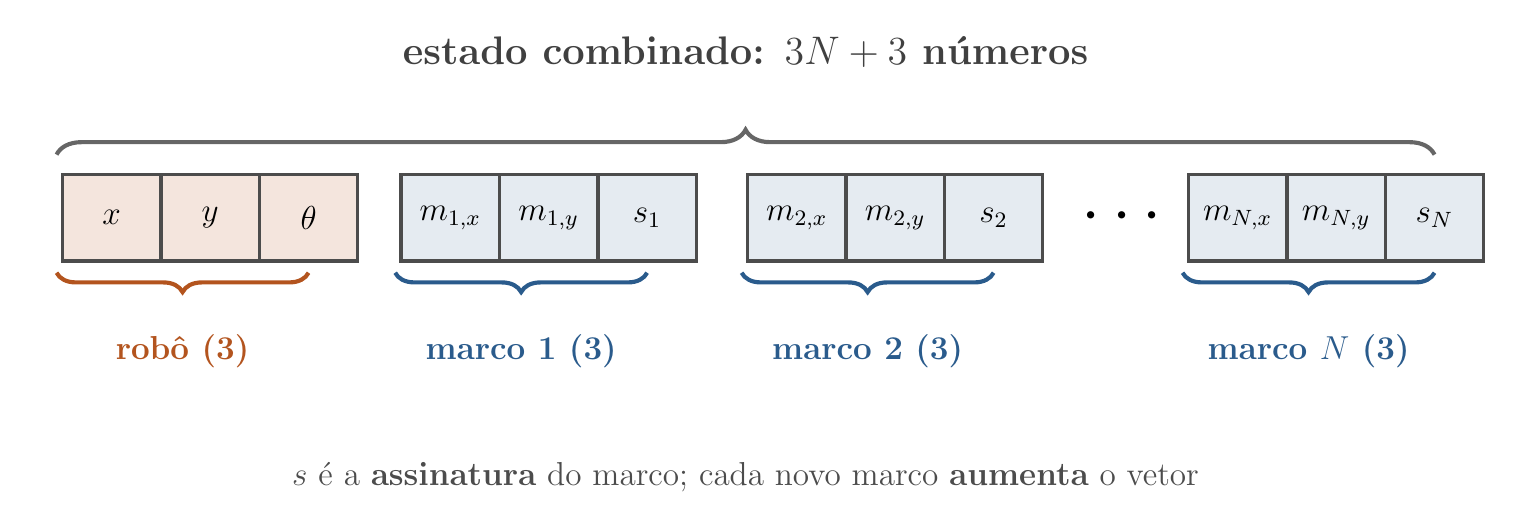
\begin{tikzpicture}[x=1cm,y=1cm]
\tikzset{k/.style={draw=black!70, line width=1.2pt, minimum width=1.25cm, minimum height=1.1cm, font=\large, inner sep=1pt, fill=white}}
\foreach \c/\t in {0/$x$,1/$y$,2/$\theta$} {\node[k, fill=dorange!15] (r\c) at ({0.7+\c*1.25},4.2) {\t};}
\foreach \c/\t in {0/$m_{1,x}$,1/$m_{1,y}$,2/$s_1$} {\node[k, fill=dblue!12] (u\c) at ({5.0+\c*1.25},4.2) {\t};}
\foreach \c/\t in {0/$m_{2,x}$,1/$m_{2,y}$,2/$s_2$} {\node[k, fill=dblue!12] (v\c) at ({9.4+\c*1.25},4.2) {\t};}
\node[font=\Huge] at (13.6,4.2) {$\cdots$};
\foreach \c/\t in {0/$m_{N,x}$,1/$m_{N,y}$,2/$s_N$} {\node[k, fill=dblue!12] (w\c) at ({15.0+\c*1.25},4.2) {\t};}
\draw[decorate, decoration={brace, amplitude=7pt, mirror}, dorange, line width=1.5pt] (0.0,3.5) -- (3.2,3.5);
\node[font=\large\bfseries, dorange] at (1.6,2.5) {robô (3)};
\draw[decorate, decoration={brace, amplitude=7pt, mirror}, dblue, line width=1.5pt] (4.3,3.5) -- (7.5,3.5);
\node[font=\large\bfseries, dblue] at (5.9,2.5) {marco 1 (3)};
\draw[decorate, decoration={brace, amplitude=7pt, mirror}, dblue, line width=1.5pt] (8.7,3.5) -- (11.9,3.5);
\node[font=\large\bfseries, dblue] at (10.3,2.5) {marco 2 (3)};
\draw[decorate, decoration={brace, amplitude=7pt, mirror}, dblue, line width=1.5pt] (14.3,3.5) -- (17.5,3.5);
\node[font=\large\bfseries, dblue] at (15.9,2.5) {marco $N$ (3)};
\draw[decorate, decoration={brace, amplitude=9pt}, black!60, line width=1.5pt] (0.0,5.0) -- (17.5,5.0);
\node[font=\Large\bfseries, black!75] at (8.75,6.3) {estado combinado: $3N + 3$ números};
\node[font=\large, black!70, text width=18cm, align=center] at (8.75,0.9) {$s$ é a \textbf{assinatura} do marco; cada novo marco \textbf{aumenta} o vetor};
\end{tikzpicture}
\end{document}
